\documentclass[notes=hide]{beamer}
\usetheme{Boadilla}

\usepackage{hyperref}
\usepackage{tikz}
\usetikzlibrary{arrows,backgrounds,positioning,fit,shapes}

\setbeamercovered{transparent}
\setbeamertemplate{enumerate items}[default]

\title{Program Synthesis}
\subtitle{Fundamentals and Applications}
\author{Rodrigo Bernardo}
\institute[]{Instituto Superior Técnico \and OutSystems \and INESC-ID}
\date{\today}

\begin{document}

\begin{frame}
  \titlepage{}
\end{frame}

\begin{frame}{Contents}
  \tableofcontents
  \note{
    Vou dar uma visão geral do que é a síntese de programas.\\
    Vou dar um exemplo muito simples.\\
    Falar das abordagens mais típicas (e simples, por isso é que são\\
    "fundamentos").\\
    De como é que isso se vai enquadrar na minha tese.\\
    E terminar com duas demonstrações de síntese.}
\end{frame}

\section{Introduction}
\subsection{What is Program Synthesis?}

\begin{frame}{\secname}{\subsecname}
  \begin{definition}<+->
    Given a specification $\phi{}$, find a program $P$ that satisfies it for all
    input $x$: $\exists{P} \ldotp \forall{x} \ldotp \phi{}(P, x)$.
  \end{definition}

  \begin{block}{Pnueli (ex-computer scientist, Turing Award)}<+->
    ``One of the most central problems in the theory of programming.''
  \end{block}

  \begin{block}{Holy Grail of Computer Science}<+->
    Decouple the \textit{what} from the \textit{how}: tell the computer what to
    do and let it figure out how to do it.
  \end{block}

  \note{
    Dada uma especificação, queremos encontrar um programa que satisfaça essa
    especificação.\\
    Aqui a especificação é dada como um predicado sobre um par (programa,
    input).\\
    Meta-objectivos: eficiência, interpretabilidade, fácil de verificar.\\
    E porquê que isto é interessante?\\
    Ora, porque num mundo perfeito gostaríamos de ordenar que o computador
    fizesse o que queremos sem termos de nos preocupar em dizer como.\\
    Para entendermos como é que esta interacção se poderia processar.
    consideremos uma interacção hipotética entre o utilizador e o sintetizador.\\}
\end{frame}

\subsection{Simple Example: Sorting}

\begin{frame}[fragile]{\secname}{\subsecname}
\begin{semiverbatim}
sort: (xs: List Int) -> (xs': List Int)
sort([])    = []
sort(x::xs) = insert(x, sort(xs))

insert: (x: Int, xs: List Int) -> (xs': List Int)
insert(x, [])    = [x]
insert(x, y::ys) = if x <= y then (x::y::ys)
                             else y::insert(x, ys)
\end{semiverbatim}
\end{frame}

\begin{frame}[fragile]{\secname}{\subsecname}
\begin{semiverbatim}
isSorted: List Int -> Bool
isSorted([])       = True
isSorted([x])      = True
isSorted(x::y::ys) = x <= y and isSorted(y::ys)
\end{semiverbatim}
\end{frame}

\begin{frame}[fragile]{\secname}{\subsecname}
\begin{semiverbatim}
sort: (xs: List Int) -> (xs': List Int)
sortSpec: isSorted(xs')

insert: (x: Int, xs: List Int) -> (xs': List Int)
insertSpec: isSorted(xs) ==> isSorted(xs')
\end{semiverbatim}
\end{frame}

\begin{frame}[fragile]{\secname}{\subsecname}
\begin{semiverbatim}
sort: (xs: List Int) -> (xs': List Int)
sort(xs) = []

insert: (x: Int, xs: List Int) -> (xs': List Int)
insert(x, xs) = []
\end{semiverbatim}
\end{frame}

\begin{frame}[fragile]{\secname}{\subsecname}
\begin{semiverbatim}
sort: (xs: List Int) -> (xs': List Int)
sortSpec: isSorted(xs') and sameContents(xs, xs')

insert: (x: Int, xs: List Int) -> (xs': List Int)
insertSpec: isSorted(xs) ==>
  isSorted(xs') and sameContents(xs', x::xs)
\end{semiverbatim}
\end{frame}

\note{Quais são as diferentes formas de expressar ao sintetizador a nossa
  intenção?}

\section{How to Express Intent}

\subsection{Specifications}

\begin{frame}{\secname}{\subsecname}
  \begin{itemize}
  \item<+-> Logical specifications
    \begin{itemize}
    \item Pre/post-conditions
    \item Loop invariants and assertions
    \item Angelic execution
    \end{itemize}
  \item<+-> Components (libraries, types)
  \item<+-> Inductive
    \begin{itemize}
    \item Input-output examples   % Idea: Flash Fill
    \item Demonstrations (traces) % Idea: emacs macro gif
    \end{itemize}
  \item<+-> Reference programs (partial/complete)
  \item<+-> Syntactic Bias
    \begin{itemize}
    \item Context-free Grammars
    \item Sketching
    \end{itemize}
  \end{itemize}
  \note{
    Eficiência, reverse engineering.\\
    Podemos ter outros casos menos típicos como, por exemplo, inferir LaTeX
    ou páginas HTML a partir de mock-ups.
    É de notar que nada impede de utilizar múltiplas formas de especificação,
    que nada mais são do que formas de restringir o espaço de procura que
    consiste em todos os programas possíveis.
  }
\end{frame}

\section{How to Find the Program}

\note{Como é que os sintetizadores realmente funcionam? Que técnicas é que o
  sintetizador utiliza para poder encontrar o programa?}

\subsection{Search Methods}

\begin{frame}{\secname}{\subsecname}
  \begin{itemize}
  \item<+-> Deductive
    \begin{itemize}
    \item Equivalence reduction rules
    \item Theorem Proving
    \end{itemize}
  \item<+-> Enumerative
    \begin{itemize} % Example: $A^{*}$
    \item Exhaustive search
    \item Best-first search
    \item Branch-and-bound
    \end{itemize}
  \item<+-> Stochastic
    \begin{itemize} % Example: STOKE
    \item Random search: Sampling, genetic programming, etc.
    \item Ranking functions
    \item Neural networks
    \end{itemize}
  \item<+-> Constraint-Solving
    \begin{itemize}
    \item Automated theorem proving % Example: SAT/SMT solvers. Show a
      % program in SMT-LIB format
    \item Solver-aided programming  % Example: Rosette, PROSE
    \end{itemize}
  \end{itemize}
  \note{
    Representa os programas numa teoria lógica como lógica de primeira ordem ou
    funções não interpretadas. A partir de uma especificação escrita nessa
    lógica, aplica os axiomas e regras de reescrita de forma a provar que a
    especificação pode ser satisfeita. A partir da prova, gera o programa.\\
    Questão: qual é o problema das NNs? Resposta: Os programas não têm uma
    interpretação óbvia. Graph NNs\\
    Geralmente, são mais utilizadas para gerar funções de custo que guiam
    procuras enumerativas. Por exemplo, elaborar heurísticas para A*.\\
    Some combination of the above.\\
    ATP: Codificar programas e especificações em formatos sobre os quais solvers
    de SAT ou SMT possam raciocinar de tal forma que as provas resultantes
    possam ser descodificadas de volta em programas.\\
    SAP: Por outro lado, SAP consiste em criar novas linguagens de programação
    que disponibilizam ao programador primitivas de alto nível como síntese,
    verificação, depuração automática e/ou execução angélica.}
\end{frame}

\subsection{Oracle-Guided Synthesis (OGIS)}

\begin{frame}{\secname}{\subsecname}
  General framework for program synthesis
  \begin{figure}[htb]
    \centering
    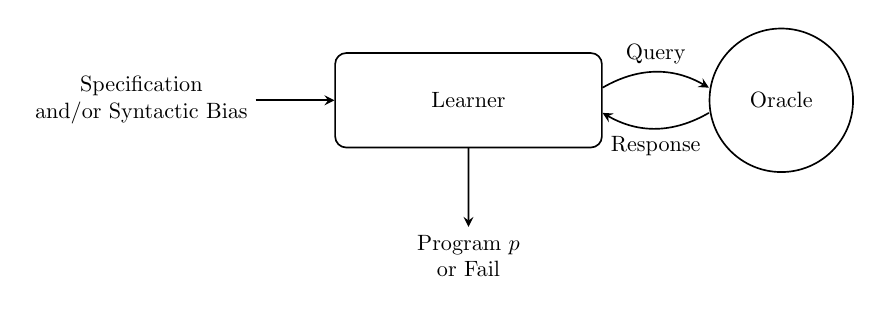
\begin{tikzpicture}
      [semithick, >=stealth, auto,
      rectangular/.style={rectangle, draw, rounded corners, text width=4cm,
        align=center, minimum size=1.5cm},
      spherical/.style={circle, draw, text width=2cm, align=center},
      scale=0.8, every node/.style={scale=0.8}]

      \onslide<2->{\node [rectangular] (S)  {Learner};}

      \onslide<3->{\node [left=1cm of S, align=center] (I) {Specification\\and/or Syntactic Bias}
        edge [->] (S);}

      \onslide<3->{\node [below=1cm of S, align=center] {Program $p$\\or Fail}
        edge [<-] (S);}

      \onslide<4->{\node [spherical] (V)  [right=1.35cm of S] {Oracle}
        ([yshift=0.2cm]S.east) edge [->, bend left]  node        {Query}    ([yshift=0.2cm]V.west)
        ([yshift=-.2cm]S.east) edge [<-, bend right] node [swap] {Response} ([yshift=-.2cm]V.west);}
    \end{tikzpicture}
  \end{figure}
  \note{De uma forma ou de outra, todos os sintetizadores que eu conheço se
    enquadram nesta framework.\\
    Que é composta por...\\
    Oráculo é onde costuma estar a componente de constraint-solving.\\
    Learner e oráculo comunicam num ciclo query-response, que tal como o nome
    indica, significa que o learner faz perguntas ao oráculo e o oráculo
    responde.}
\end{frame}

\begin{frame}{\secname}{\subsecname: Queries/Responses}
  \begin{itemize}[<+->]
  \item Membership: \textit{Is $(I,O)$ a positive example?}
  \item Positive/negative witness: \textit{Give me a positive/negative example.}
  \item Counterexample: \textit{I have program $P$. Give me a positive example
      that it does not satisfy.}
  \item Correctness: \textit{Is $P$ the program you want?}
  \item Distinguishing input: \textit{I have program $P$. Give me a new program
      that satisfies all the examples that $P$ does plus a counterexample to
      $P$.}
  \end{itemize}
  \note{O interesse nesta framework está precisamente no tipo de perguntas a
    que o oráculo consegue responder. Quanto mais fracas as perguntas, mais
    forte o sintetizador.\\
    Algumas das mais interessantes são:
    Membership: filiação\\
    Witness: testemunha\\
    Distinguishing: diferenciador}
\end{frame}

\section{Thesis}

\begin{frame}{\secname}
  Setting is programming by examples:
  \begin{itemize}
  \item Maybe add sketching features
    \note{Programas parciais/templates com buracos.\\}
  \item Simple interface
    \note{Ideia intuitiva, simples, e muitos dos casos de interesse podem ser
      descritos desta forma.\\}
  \item Underspecification
    \note{Ambiguidade: Há muitos programas (infinitos, possivelmente) que
      satisfazem os exemplos, mas em qual deles é que o utilizador está a
      pensar?\\}
    \onslide<2->{
      \begin{enumerate}
      \item Ranking
      \item Display the program to the user
      \item Accept more examples
      \item Show distinguishing inputs
      \item Accept negative examples
      \end{enumerate}}
    \note{Prever o que o utilizador quer.\\
      Deixar a decisão para o utilizador.\\
      Trivial.\\
      Exemplos que desambiguam dois programas.\\
      Exemplos que o programa não deve satisfazer.\\}
   \end{itemize}
\end{frame}

\section{Demonstration}

\begin{frame}{\secname}
  \begin{itemize}
  \item \href{https://microsoft.github.io/prose/}{PROSE}
    \note{PBE; focused on Data Wrangling}
  % \item \href{https://github.com/fredfeng/Tyrell}{Tyrell}
  %   \note{Mais geral. Permite programar enumeradores e oráculos para criar
  %     os nossos próprios sintetizadores. Muito mais recente.}
  \end{itemize}
\end{frame}

\section{Discussion Topic}

\begin{frame}{\secname}
  \begin{itemize}
  \item Difference between program synthesis and compilation
  \item Difference between program synthesis and machine learning
  \item Verification of machine learning systems, explainable AI
    \begin{itemize}
    \item In general: bridge between machine learning and formal methods
    \end{itemize}
  \end{itemize}
\end{frame}

\end{document}
